%%%%%%%%%%%%%%%%%%%%%%%%%%%%%%%%%%%%%%%%%%%%%%%%%%%%%%%%%%%%%%%%%%%%%%%%%%%%%%%%
% TUM-Vorlage: Präsentation - Beispiele
%%%%%%%%%%%%%%%%%%%%%%%%%%%%%%%%%%%%%%%%%%%%%%%%%%%%%%%%%%%%%%%%%%%%%%%%%%%%%%%%


%%%%%%%%%%%%%%%%%%%%%%%%%%%%%%%%%%%%%%%%%%%%%%%%%%%%%
%% Folie: Gültigkeit der Masterfolien              %%
%%%%%%%%%%%%%%%%%%%%%%%%%%%%%%%%%%%%%%%%%%%%%%%%%%%%%

%%%%%%%%%%%%%%%%%%%%%%%%%%%%%%%%%%%%%%%%%%%%%%%%%%%%%
%% Folie: Grundlage der Masterfolien               %%
%%%%%%%%%%%%%%%%%%%%%%%%%%%%%%%%%%%%%%%%%%%%%%%%%%%%%

%%%%%%%%%%%%%%%%%%%%%%%%%%%%%%%%%%%%%%%%%%%%%%%%%%%%%
%% Folie: 2-zeilige Überschrift                    %%
%%%%%%%%%%%%%%%%%%%%%%%%%%%%%%%%%%%%%%%%%%%%%%%%%%%%%


\begin{frame}
\shiftedframetitle{Motivation}

\begin{itemize}
    \itemsep2em
    \item Web latency and security are becoming more and more important.
    
    \item Middleboxes have caused a protocol ossification. Attempted extensions to TCP like TCP Fast Open\cite{DBLP:conf/conext/RadhakrishnanCCJR11}, SCTP\cite{rfc3286}, Multipath TCP \cite{rfc6824} have not seen widespread deployment.
    
    \item QUIC is a user-space transport protocol built on top of UDP. Also QUIC provides for authenticated, encrypted header and payload which avoids dependency on vendors
    and ISPs
    
    %\item Google started work on QUIC in 2012. 
    
    \item Faster development and deployment cycles. Already on Q044 version and accounts for more than 35\% of
    Google’s total egress traffic and 7\% of global internet traffic.
    
    \item  QUIC has been shown to reduce search latency by 8\% for desktop users and 3.6\% for mobile users.\cite{DBLP:conf/sigcomm/LangleyRWVKZYKS17}
    
    %\item An IETF working group has been
    %formed to standardize QUIC which should lead to even greater adoption.
    
\end{itemize}
\end{frame}
\clearpage


\begin{frame}
\shiftedframetitle{Goal and Approach}
\begin{itemize}
    \itemsep2em
    \item Initial performance results from Google showed improvements in latency, rebuffer rates and lower packet loss rates but there is still a lack
    of repeatable studies.
    
    \item Rapid development cycle of QUIC means
    that many new features are introduced in each version of QUIC and support for older
    versions is dropped. So previous studies(refer Prior Work) become obsoleted quickly.
    
    \item In this thesis we aim to evaluate the performance of QUIC(Q035, Q039, Q043, Q044) and compare it with
    TCP/TLS. 
    
    \item To do this we conduct experiments on real scenarios rather than in an emulated environment to investigate connection establishment time, Time to first byte, download time, YouTube QoE metrics, Throughput,
    fairness in competing flow scenarios and CPU utilization.
    
\end{itemize}
\end{frame}
\clearpage

\begin{frame}
    \shiftedframetitle{Goal and Approach}
    \begin{itemize}
        \itemsep3em 
        \item\textbf{RQ1 : How do different versions of QUIC compare with each other and TCP/TLS 1.2 and TCP/TLS 1.3 on IPv4 and IPv6?}
% Newer versions of QUIC(Q044) should ideally provide some improvement over older ones(Q043, Q039, Q035).
        
        \item\textbf{RQ2 : How do the versions of QUIC compare with each other on different Autonomous Systems?}

        \item\textbf{RQ3 : How does throughput and CPU utilization of QUIC compare with TCP/TLS?}
        
        
        \item\textbf{RQ4 : Is QUIC fair towards TCP/TLS in sharing bandwidth?}
        
    \end{itemize}
\end{frame}
\clearpage



%\begin{frame}
%\shiftedframetitle{Background}
%SPDY is the first attempt by Google to improve Web Latency.\cite{spdy} HTTP/2 is the successor of SPDY protocol.
%
%It has features like multiplexing requests over a single TCP connection, HTTP header compression, request prioritization, server push and server hint\cite{rfc7540}
%
%HTTP/2 suffers from the TCP head-of-line blocking issue.
%
%Previous work \cite{DBLP:conf/networking/El-khatibTW14}\cite{7745823}\cite{DBLP:conf/sac/CarlucciCM15}\cite{DBLP:conf/icc/MegyesiKM16} shows the improvements provided by SPDY and HTTP/2.  
%
%    QUIC has many innovative features like Version Negotiation, 0-RTT connection establishment, Reduced head-of-line blocking, improved congestion control using packet pacing, Authenticated, encrypted header and payload, stream multiplexing, Connection-IDs, stream and connection level flow control, connection migration and resilience to NAT rebinding.\cite{ietf-quic-transport-18}
%
%\end{frame}
%\clearpage

\begin{frame}
    \shiftedframetitle{Background}
QUIC replaces most of the traditional HTTPS stack: TCP, TLS, HTTP/2.
\begin{figure}[!t]
    
    \minipage{0.7\textwidth}
    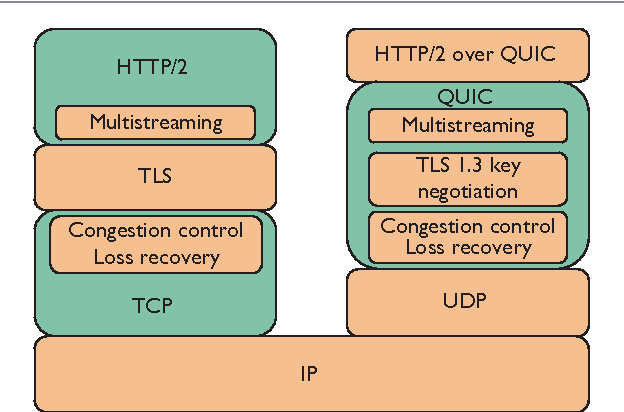
\includegraphics[width=1\textwidth]
    {figures/QUICstack.png}
    \endminipage\hfill
    \caption{\label{fig:QUIC_architecture}Layered QUIC architecture in the traditional HTTPS stack. QUIC incorporates features of congestion control, loss recovery similar to TCP, Multiple streams like HTTP2 and key negotiation like TLS.\cite{Cui2017}}
    
\end{figure}
\end{frame}
\clearpage

\begin{frame}
    \shiftedframetitle{Connection Establishment\cite{DBLP:conf/sigcomm/LangleyRWVKZYKS17}\cite{quicgd}\cite{crypto}}
    
    \begin{figure}[!ht]
        
        \minipage{0.7\textwidth}
        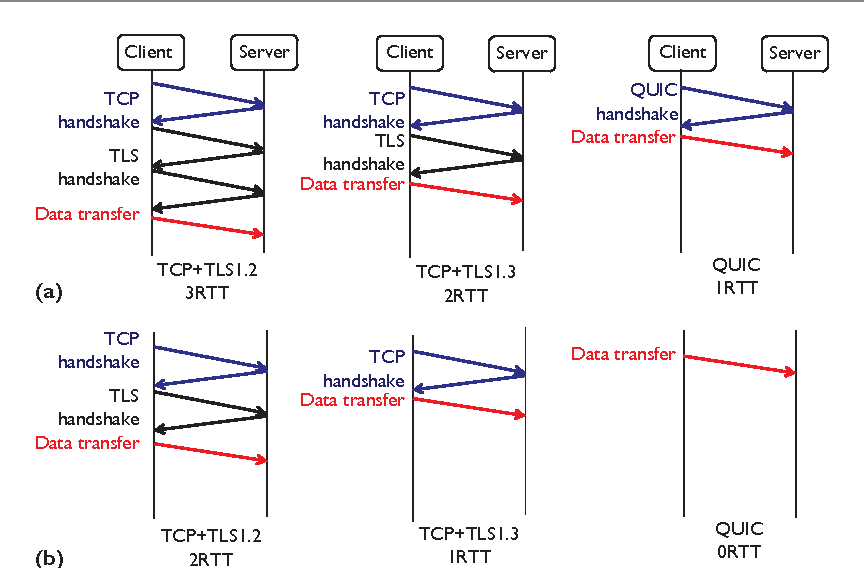
\includegraphics[width=1\textwidth]
        {figures/0rtt.png}
        \endminipage\hfill
        \caption{\label{fig:RTT} Handshake round-trip time (RTT) of different protocols. (a) First-time connection establishment. (b) Subsequent connections.\cite{Cui2017}}
    \end{figure}

    
    
\end{frame}
\clearpage

%\begin{frame}
%    \shiftedframetitle{Multiplexing}
%    \begin{figure}[!ht]
%        
%        \minipage{0.6\textwidth}
%        \includegraphics[width=1\textwidth]
%        {figures/hol.png}
%        \endminipage\hfill
%        \caption{\label{fig:hol}Multiplexing comparison. This involved sending multiple streams of data over a single transport connection using (a) HTTP1.1, (b) HTTP/2, and (c) QUIC.\cite{Cui2017}}
%    \end{figure}
%
%QUIC also supports multiple streams in a single connection but the packets can be delivered out of order and a lost packet affects only those streams whose data it carried, not affecting other streams.
%
%
%\end{frame}
%\clearpage
%
%\begin{frame}
%    \shiftedframetitle{Congestion Control + Packet Pacing}
%    
%        \begin{figure}[!ht]
%        
%        \minipage{0.7\textwidth}
%        \includegraphics[width=1\textwidth]
%        {figures/pacing.png}
%        \endminipage\hfill
%        \caption{\label{fig:pacing}Packet Pacing \cite{DBLP:conf/ipccc/YuXY17}}
%    \end{figure}
%
%Default congestion control algorithm is CUBIC\cite{DBLP:journals/internet/CuiLLWK17} but differs from TCP CUBIC slightly.\cite{quicgd}\cite{ietf-quic-recovery-18}. BBR is a new congestion control algorithm being developed by Google.\cite{DBLP:conf/pam/LiCJC18}
%
%Packet Pacing is done by inserting a waiting time between each UDP datagram (enabled by default)
%This helps lower retransmission rate \cite{DBLP:conf/infocom/AggarwalSA00}
%
%\end{frame}
%\clearpage

%\begin{frame}
%\shiftedframetitle{Prior Work}\label{prior_work}
%    Langley et al. \cite{DBLP:conf/sigcomm/LangleyRWVKZYKS17} discuss about motivations in various design decisions of QUIC, development and testing performed over various iterations, performance improvements. They provide us with the first large-scale measurements of QUIC across various versions.
%    
%    Nepomuceno et al.\cite{8538687}, Cook et al.\cite{DBLP:conf/icc/CookMTH17} look at page load time.
%    
%    Li et al.\cite{DBLP:conf/pam/LiCJC18}, Kharat et al.\cite{8524247}, Qian et al. \cite{DBLP:journals/access/QianWT18}, Kakhki et al.\cite{DBLP:conf/imc/KakhkiJCNM17}look at throughput, congestion control and fairness among flows.
%    
%    Yu et al. \cite{DBLP:conf/ipccc/YuXY17} focused mainly on packet pacing mechanism for congestion control.
%    
%    Saverimoutou et al.\cite{DBLP:conf/iscc/SaverimoutouMV17}, Fischlin et al.\cite{DBLP:conf/ccs/FischlinG14} and Vaere et al.\cite{DBLP:conf/imc/VaereBKT18} look into the security aspects of QUIC.
%    
%    Willem et al.\cite{udpgso} and Edeline et al. \cite{DBLP:journals/corr/EdelineKTAD16} look into how QUIC being built on top of UDP affects it.
%    
%    Wang et al.\cite{DBLP:conf/mswim/WangBRP18} implement QUIC in the linux kernel and perform experiments to compare both in kernel mode.
%
%    Rüth et al.\cite{DBLP:conf/pam/RuthPDH18} look into QUIC usage in the wild.
%
%     
%\end{frame}
%\clearpage

\begin{frame}
\shiftedframetitle{Methodology}
    \begin{itemize}
    \itemsep3em 

%We look at metrics like connection establishment time(For QUIC this will be 1-RTT Handshake, for TCP/TLS1.3 2-RTT and for TCP/TLS1.2 3-RTT), time to first byte and page download time using \texttt{quic\_perf} and \texttt{tls\_perf}.
    \item connection establishment time, time to first byte and page download time %using \texttt{quic\_perf} and \texttt{tls\_perf}.

    \item Analyze these metrics on AS level(announces prefix of our target websites) %using RIPE Database.\cite{RIPEDB} 

    \item YouTube QoE metrics like Connect Time to media CDNs, Prebuffering time, Startup delay and Overall download %rate using \texttt{YouTube tests}

    \item Throughput and  CPU utilization %using \texttt{YouTube tests}, \texttt{quic\_perf} and \texttt{tls\_perf}.

%CUBIC congestion control fairness in cases of competing flows by running the tests concurrently.
    \item Congestion control fairness in cases of competing flows
%We use \texttt{perf} and \texttt{strace} to profile QUIC and explain its high CPU utilization.
    \item \texttt{perf} and \texttt{strace} to profile QUIC
%We investigate QUIC Discovery using Alt-Svc Header
\end{itemize}
 
\end{frame}
\clearpage

\begin{frame}
    \shiftedframetitle{Methodology}
\begin{itemize}
\itemsep3em 
\item Reused the \texttt{YouTube test} for TCP developed by S Ahsan et al.\cite{DBLP:conf/pam/AhsanBOS15} which was modified to use QUIC by Sergey\cite{sergey} and \texttt{tls\_perf} and \texttt{\texttt{quic\_perf}} by Bernhard\cite{bernhard}. Several additions and improvements were made to their tests like adding support for Q044, improving logging and error handling, adding HTTP/2 support.

\item Used the latest version of \texttt{litespeed lsquic client}\footnote[frame]{https://github.com/litespeedtech/lsquic-client/tree/1.17.8} and \texttt{Boringssl} library for QUIC implementation.

\item \texttt{libcurl} was used for TCP implementation.

\item For measurements over IETF QUIC we used the QUIC Tracker \cite{quic_tracker} test suite which supports QUIC(draft-17) and is also TLS1.3 compatible.

%Created debian packages using cpack for easier deployment over Raspberry PI.
%
%List of target websites for our measurements was taken from QUIC Research@COMSYS\cite{comsys}
%
%Top 50 most popular videos for a region were selected for measurements over YouTube and files of different sizes were uploaded to Google Drive for performance tests
\end{itemize}
\end{frame}
\clearpage

\begin{frame}
    \shiftedframetitle{Measurement Setup}
\begin{itemize}
\itemsep3em
\item Measurements were performed from 3 vantage Points.  

\item VM \texttt{vmott16.cm.in.tum.de} with linux OS. Bandwidth: 400 Mbits/s
It supported both IPv4 and IPv6.
%This machine has over 400 Mbits/s UDP connection speed with Microsoft Azure virtual
server and 1.20 Gbits/s via TCP. 

\item Raspberry Pi 3 Model B with 1 GB RAM and 32 GB microSDHC Card. Bandwidth: 100 Mbits/s line. This PI was installed at a residential location in Munich, Germany.
% connected to a LAN network run by the Leibniz-datacenter(LRZ).

\item Another Raspberry PI was installed in Bhubaneswar, India. Bandwidth: 20 Mbits/s line but peak bandwidth was measured at 14 Mbit/s during testing. 

\item Only IPv4 could be tested at the above two locations because of lack of IPv6 support

%The tests were coded in C as libraries used provide us with an easy-to-use C API.
%The IETF test were coded in Go.
\end{itemize}
\end{frame}
\clearpage

\begin{frame}
\shiftedframetitle{Connection Establishment Times}
\begin{figure}[!htb]
    \begin{subfigure}{0.45\textwidth}
        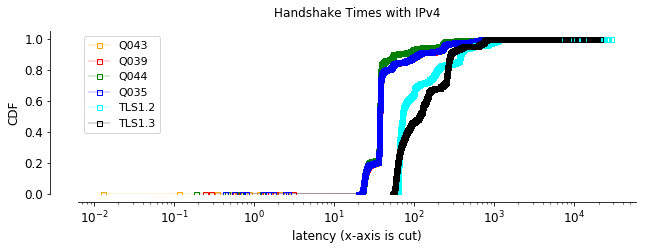
\includegraphics[width=\linewidth]{./plots/VM/handshake_times_ipv4.png}
        %\caption{CDF for IPv4.}\label{fig:cdf-of-connection}
    \end{subfigure}%
    %\caption{CDFs of Connection Times for QUIC(Q044, Q043, Q039, Q035) and TLS(TLS 1.3, TLS 1.2) for IPv4. QUIC has lower connection times than TLS. Q044 has slightly better performance than other QUIC versions}\label{fig:cdfs-of-connection4}
%\end{figure}
%\begin{figure}[!htb]
    \begin{subfigure}{0.45\textwidth}
        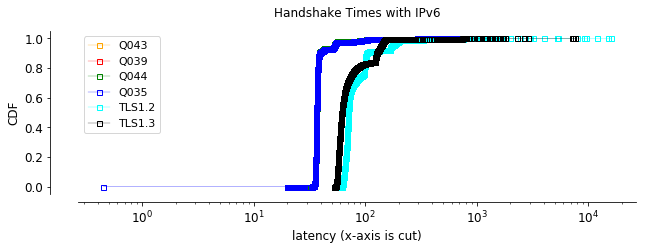
\includegraphics[width=\linewidth]{./plots/VM/handshake_times_ipv6.png}
        %\caption{CDF for IPv6}\label{fig:cdf-of-connection}
    \end{subfigure}
    %\caption{CDFs of Connection Times for QUIC(Q044, Q043, Q039, Q035) and TLS(TLS 1.3, TLS 1.2) for IPv6}\label{fig:cdfs-of-connection}
        \caption{CDFs of Connection Times for QUIC(Q044, Q043, Q039, Q035) and TLS(TLS 1.3, TLS 1.2) for Ipv4, IPv6}\label{fig:cdfs-of-connection}
\end{figure}
%\end{frame}
%\clearpage
%
%\begin{frame}
%\shiftedframetitle{Connection Establishment Times}
\begin{figure}[!htb]    
    \begin{subfigure}{0.45\textwidth}
        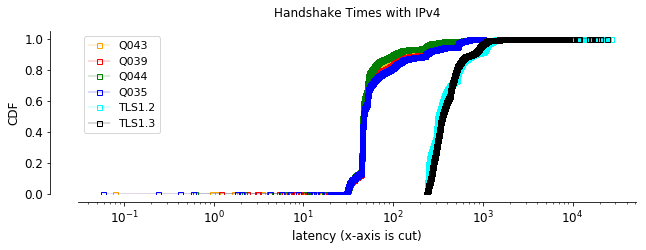
\includegraphics[width=\linewidth]{./plots/PI/handshake_times_ipv4.png}
    \end{subfigure}
%    \caption{CDFs of Connection Times for QUIC(Q044, Q043, Q039, Q035) and TLS(TLS 1.3, TLS 1.2) for IPv4 from Raspberry Pi in Munich}\label{fig:cdfs-of-connectionin}
%\end{figure}
%
%\begin{figure}[!htb]
    \begin{subfigure}{0.45\textwidth}
        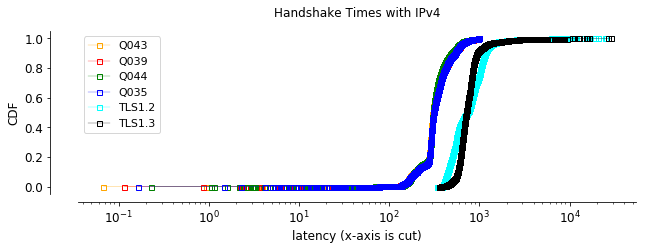
\includegraphics[width=\linewidth]{./plots/India/handshake_times_ipv4.png}
    \end{subfigure} 
    \caption{CDFs of Connection Times for QUIC(Q044, Q043, Q039, Q035) and TLS(TLS 1.3, TLS 1.2) for IPv4 from Raspberry Pi in Munich, Germany and Bhubaneswar, India}\label{fig:cdfs-of-connectionm}
\end{figure}
\end{frame}
\clearpage

\begin{frame}
\shiftedframetitle{Time to first byte}
\begin{figure}[!htb]
    \begin{subfigure}{0.45\textwidth}
        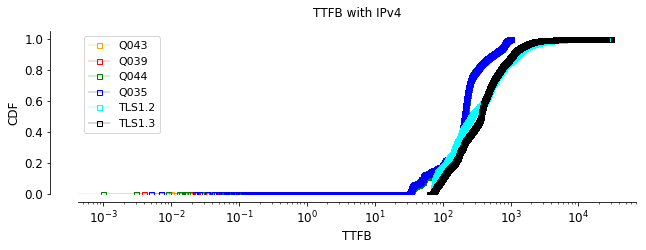
\includegraphics[width=\linewidth]{./plots/VM/TTFB_ipv4.png}
    \end{subfigure}
    \begin{subfigure}{0.45\textwidth}
        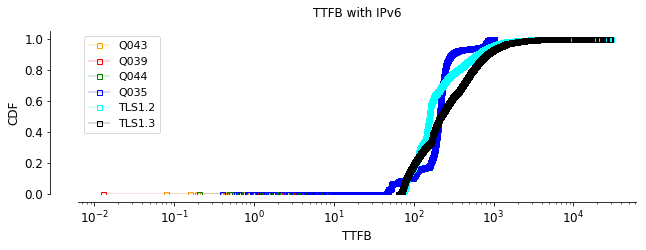
\includegraphics[width=\linewidth]{./plots/VM/TTFB_ipv6.png}
    \end{subfigure}    
    \caption{CDFs of Time to First Byte for QUIC(Q044, Q043, Q039, Q035) and TLS(TLS 1.3, TLS 1.2) for IPv4, IPv6.}\label{fig:cdf-of-time}
\end{figure}
%\end{frame}
%\clearpage
%
%\begin{frame}
%\shiftedframetitle{Time to first byte}
\begin{figure}[!htb]
    
    \begin{subfigure}{0.45\textwidth}
        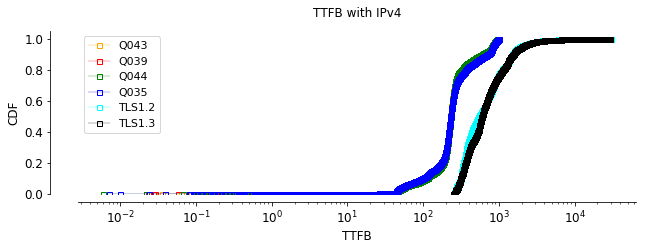
\includegraphics[width=\linewidth]{./plots/PI/TTFB_ipv4.png}
    \end{subfigure}  
%    \caption{CDFs of TTFB for QUIC(Q044, Q043, Q039, Q035) and TLS(TLS 1.3, TLS 1.2) for IPv4 from Raspberry Pi in Munich}
%\end{figure}
%
%\begin{figure}[!htb]
    \begin{subfigure}{0.45\textwidth}
        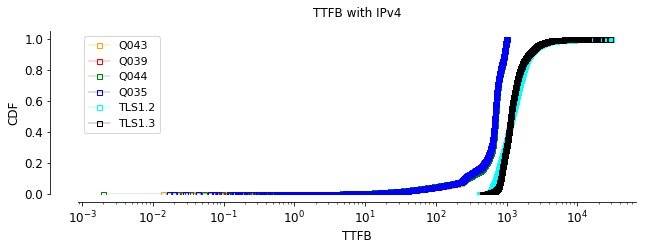
\includegraphics[width=\linewidth]{./plots/India/TTFB_ipv4.png}
    \end{subfigure}
   % \caption{CDFs of TTFB for QUIC(Q044, Q043, Q039, Q035) and TLS(TLS 1.3, TLS 1.2) for IPv4 from Raspberry Pi in India}
        \caption{CDFs of TTFB for QUIC(Q044, Q043, Q039, Q035) and TLS(TLS 1.3, TLS 1.2) for IPv4 from Raspberry Pi in Munich, Germany and Bhubaneswar, India}
\end{figure}
\end{frame}
\clearpage

%\begin{frame}
%\shiftedframetitle{AS topology}
%\begin{table}[ht]
%    \begin{tabular}{@{}|l|l|l|@{}}
%        \toprule
%        \textbf{ASNo} & \multicolumn{1}{c|}{\textbf{ASName}} & \textbf{No. of websites} \\ \midrule
%        15169 & GOOGLE - Google LLC & 3863 \\ \midrule
%        15133 & EDGECAST MCI Communications Services & 689 \\ \midrule
%        55293 & A2HOSTING - A2 Hosting & 178 \\ \midrule
%        203226 & IHCRU - Internet-Hosting Ltd & 82 \\ \midrule
%        16276 & OVH - OVH SAS & 75 \\ \bottomrule
%    \end{tabular}
%    \caption{Top-5 AS with the no. of websites in our target list. Google serves a large majority of websites over QUIC}
%    \label{table:top-5-as-with}
%\end{table}
%\end{frame}
%\clearpage


\begin{frame}
\shiftedframetitle{AS topology}
\begin{figure}[!htb] 
    \begin{subfigure}{0.45\textwidth}
        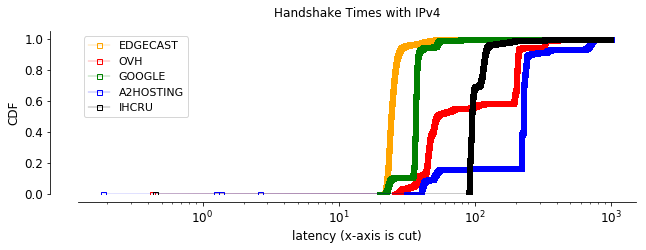
\includegraphics[width=\linewidth]{./plots/VM/handshake_times_IPv4_asno.png}
    \end{subfigure}
    \begin{subfigure}{0.45\textwidth}
        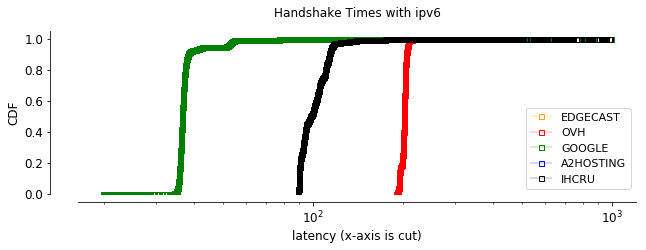
\includegraphics[width=\linewidth]{./plots/VM/handshake_times_ipv6_asno.png}
    \end{subfigure} 
    \caption{CDFs of Connection Times for all for QUIC(all versions combined) categorized by AS for IPv4, IPv6. EDGECAST performs better than GOOGLE}\label{fig:connection-times-for}
\end{figure}
%\end{frame}
%\clearpage
%\begin{frame}
%\shiftedframetitle{AS topology}
\begin{figure}[!htb] 
    \begin{subfigure}{0.45\textwidth}
        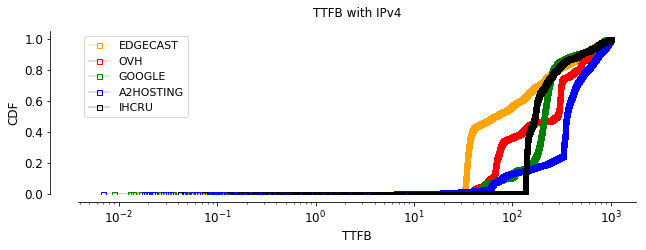
\includegraphics[width=\linewidth]
        {./plots/VM//TTFB_ipv4_asno.png}
    \end{subfigure}
    \begin{subfigure}{0.45\textwidth}
        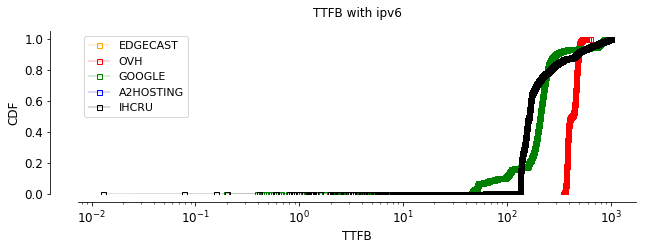
\includegraphics[width=\linewidth]
        {./plots/VM/TTFB_ipv6_asno.png}
    \end{subfigure}
    \caption{\label{fig:TTFB_ipv6_asno}CDF of Time to First Byte for QUIC(all versions combined) categorized by AS for IPv4, IPv6}
\end{figure}
Google AS serves an overwhelming majority of websites using QUIC, almost half of the websites in our target list.
\end{frame}
\clearpage
\begin{frame}
\shiftedframetitle{YouTube QoE}
\begin{figure}[!htb]
    \begin{subfigure}{0.45\textwidth}
        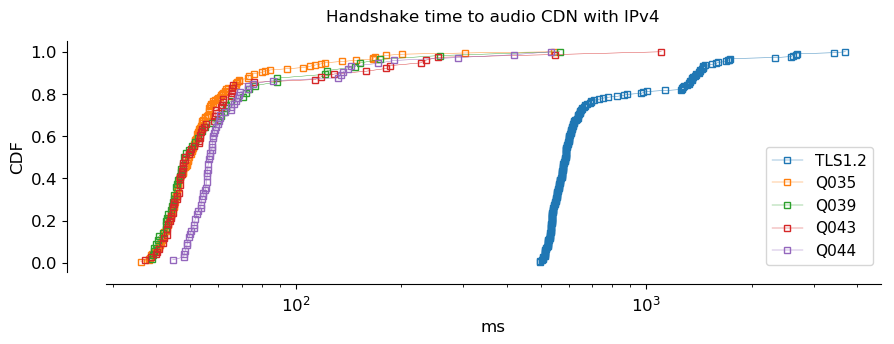
\includegraphics[width=\linewidth]{./plots/youtube/india/graph_audio_connect_time.png}
    \end{subfigure}
    \begin{subfigure}{0.45\textwidth}
        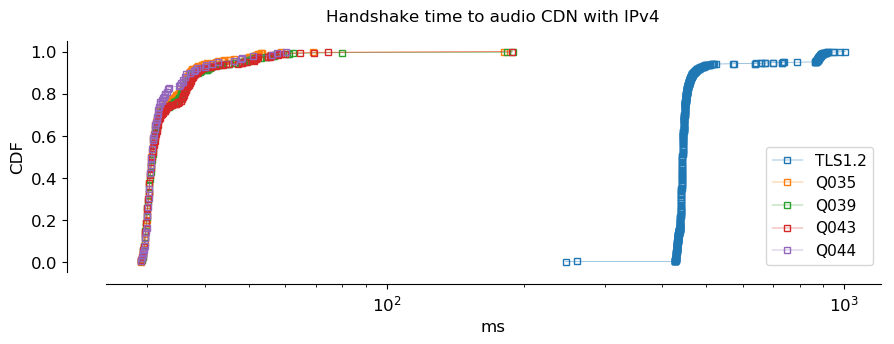
\includegraphics[width=\linewidth]{./plots/youtube/munich/graph_audio_connect_time.png}
    \end{subfigure}    
    \caption{CDF of Audio Connect Time for IPv4 in Bhubaneswar, India and Munich, Germany}\label{fig:cdf-of-audio}
\end{figure}
%\end{frame}
%\clearpage
%
%\begin{frame}
%\shiftedframetitle{YouTube QoE}
\begin{figure}[!htb]
    \begin{subfigure}{0.45\textwidth}
        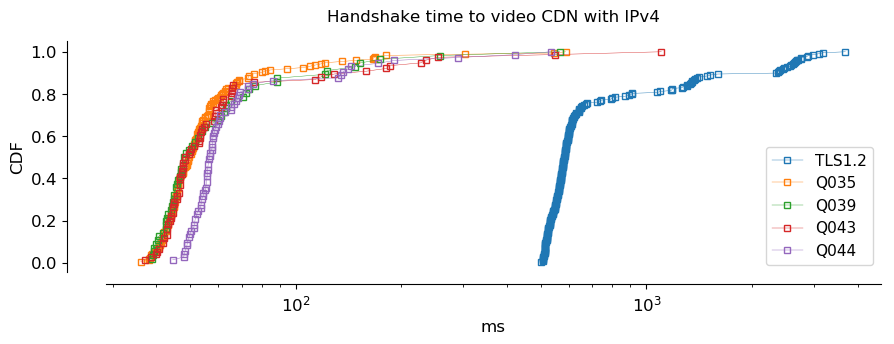
\includegraphics[width=\linewidth]{./plots/youtube/india/graph_video_connect_time.png}
    \end{subfigure}
    \begin{subfigure}{0.45\textwidth}
        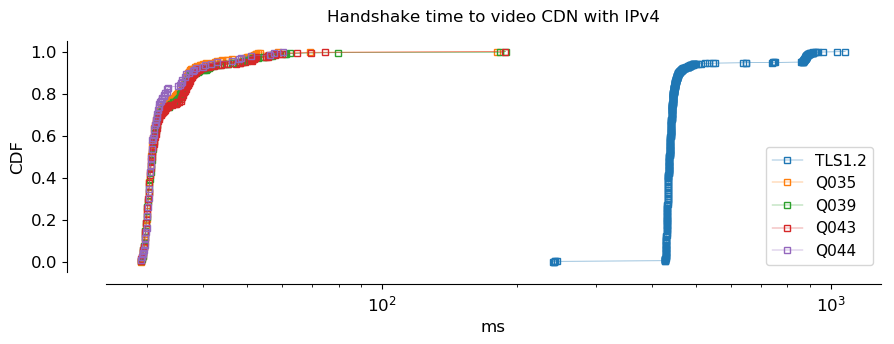
\includegraphics[width=\linewidth]{./plots/youtube/munich/graph_video_connect_time.png}
    \end{subfigure}    
    \caption{CDF of Video Connect Time for IPv4 in Bhubaneswar, India and Munich, Germany}\label{fig:cdf-of-video}
\end{figure}
\end{frame}
\clearpage

\begin{frame}
\shiftedframetitle{YouTube QoE}
%\begin{figure}[!htb]
%    \begin{subfigure}{0.45\textwidth}
%        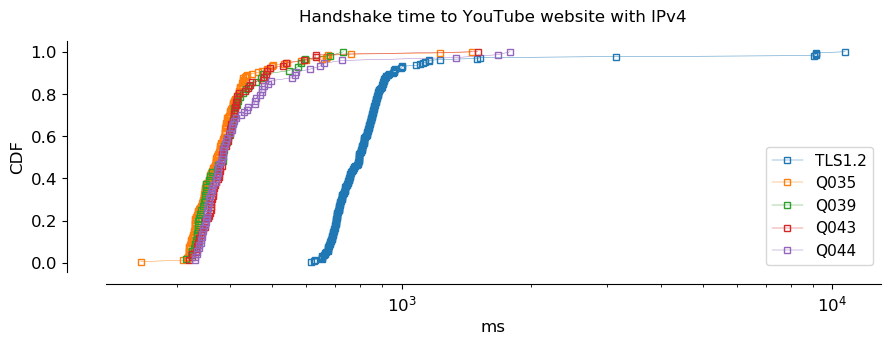
\includegraphics[width=\linewidth]{./plots/youtube/india/graph_website_connect_time.png}
%    \end{subfigure}
%    \begin{subfigure}{0.45\textwidth}
%        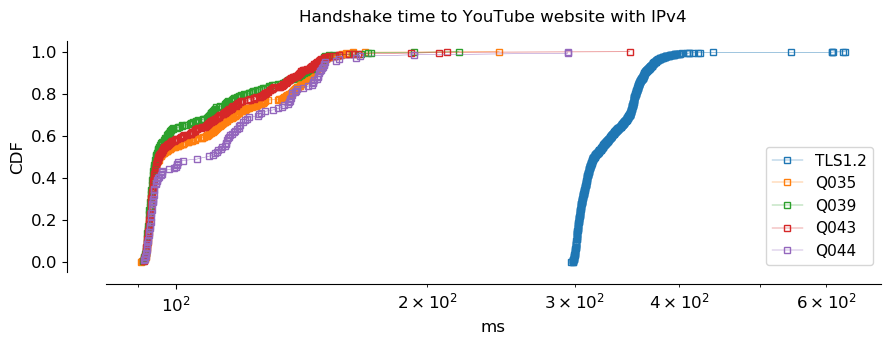
\includegraphics[width=\linewidth]{./plots/youtube/munich/graph_website_connect_time.png}
%    \end{subfigure}    
%    \caption{CDF of Website Connect Time for IPv4 in Bhubaneswar, India and Munich, Germany}
%\end{figure}
%\end{frame}
%\clearpage
%
%\begin{frame}
%\shiftedframetitle{YouTube QoE}
\begin{figure}[!htb]
    \begin{subfigure}{0.45\textwidth}
        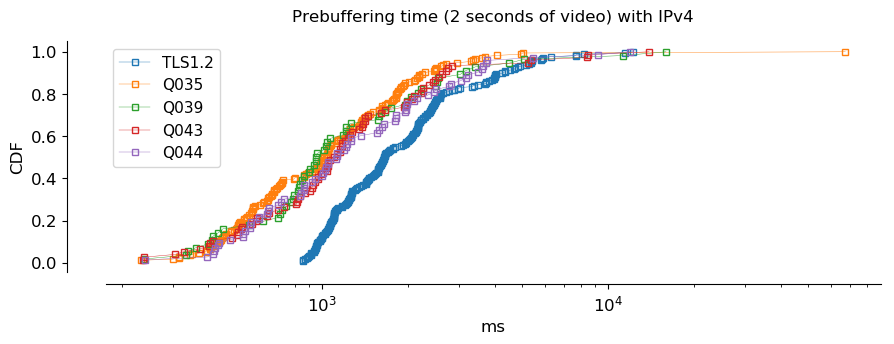
\includegraphics[width=\linewidth]{./plots/youtube/india/graph_prebuffering_duration.png}
    \end{subfigure}
    \begin{subfigure}{0.45\textwidth}
        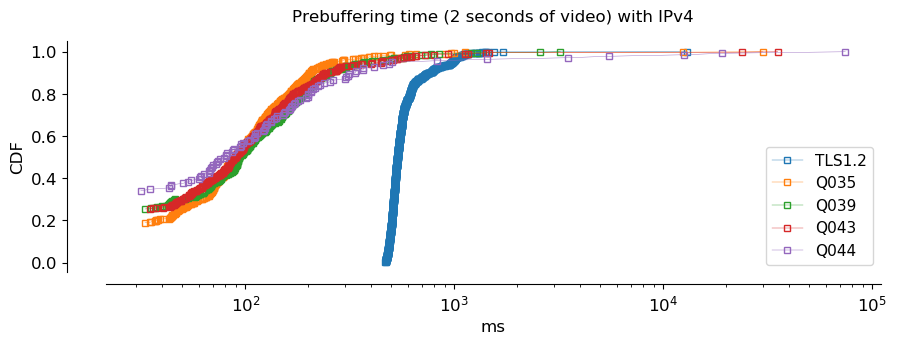
\includegraphics[width=\linewidth]{./plots/youtube/munich/graph_prebuffering_duration.png}
    \end{subfigure}    
    \caption{CDF of Prebuffering time for IPv4 in Bhubaneswar, India and Munich, Germany}\label{fig:cdf-of-prebuffering}
\end{figure}
%\end{frame}
%\clearpage
%
%\begin{frame}
%\shiftedframetitle{YouTube QoE}
\begin{figure}[!htb]
    \begin{subfigure}{0.45\textwidth}
        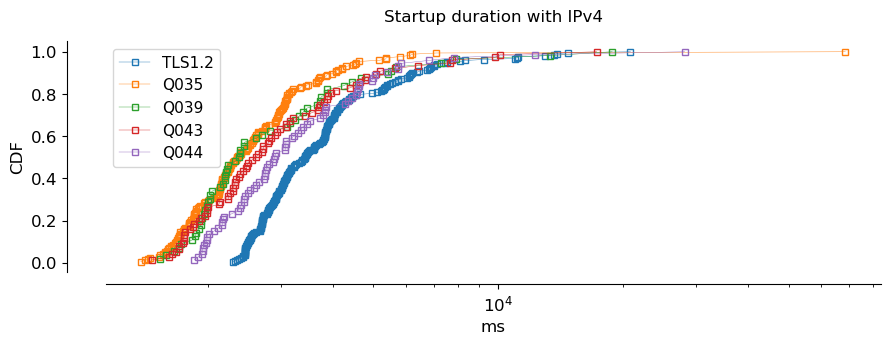
\includegraphics[width=\linewidth]{./plots/youtube/india/graph_startup_delay.png}
    \end{subfigure}
    \begin{subfigure}{0.45\textwidth}
        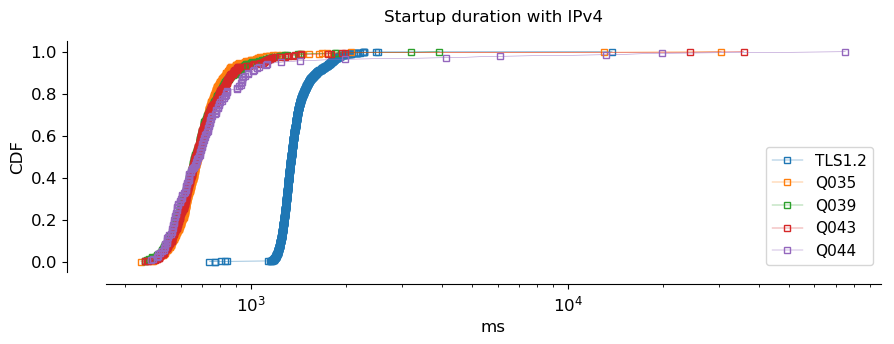
\includegraphics[width=\linewidth]{./plots/youtube/munich/graph_startup_delay.png}
    \end{subfigure}    
    \caption{CDF of startup delay for IPv4 in Bhubaneswar, India and Munich, Germany}\label{fig:cdf-of-startup}
\end{figure}

\end{frame}
\clearpage

\begin{frame}
\shiftedframetitle{YouTube QoE}

\begin{figure}[!htb]  
    \begin{subfigure}{0.45\textwidth}
        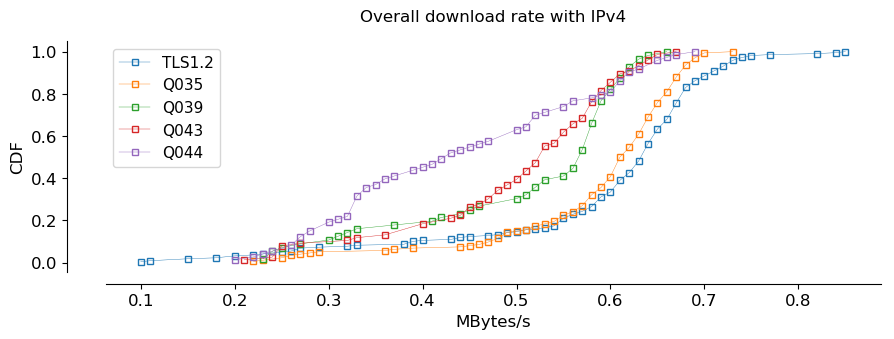
\includegraphics[width=\linewidth]{./plots/youtube/india/graph_download_rate.png}
    \end{subfigure}
    \begin{subfigure}{0.45\textwidth}
        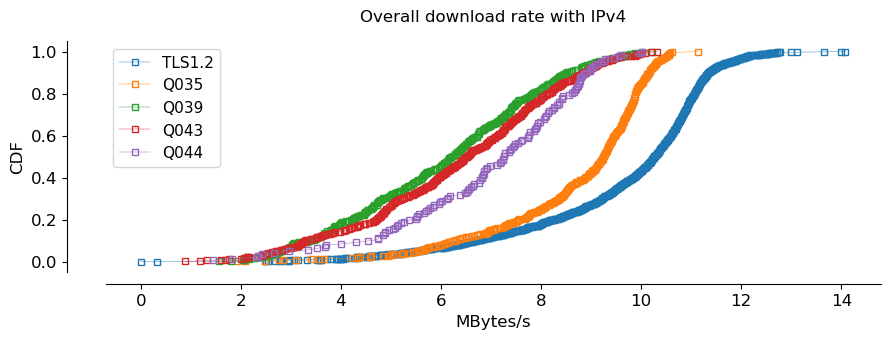
\includegraphics[width=\linewidth]{./plots/youtube/munich/graph_download_rate.png}
    \end{subfigure}    
    \caption{CDF of Download rate for IPv4 in Bhubaneswar, India and Munich, Germany}\label{fig:cdf-of-download}
\end{figure}
%\end{frame}
%\clearpage
%
%\begin{frame}
%\shiftedframetitle{YouTube QoE}
\begin{figure}[!htb]
    \begin{subfigure}{0.45\textwidth}
        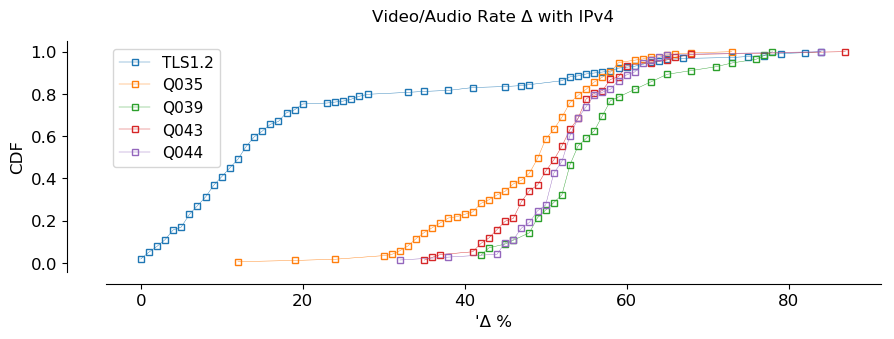
\includegraphics[width=\linewidth]{./plots/youtube/india/graph_rate_diff.png}
    \end{subfigure}
    \begin{subfigure}{0.45\textwidth}
        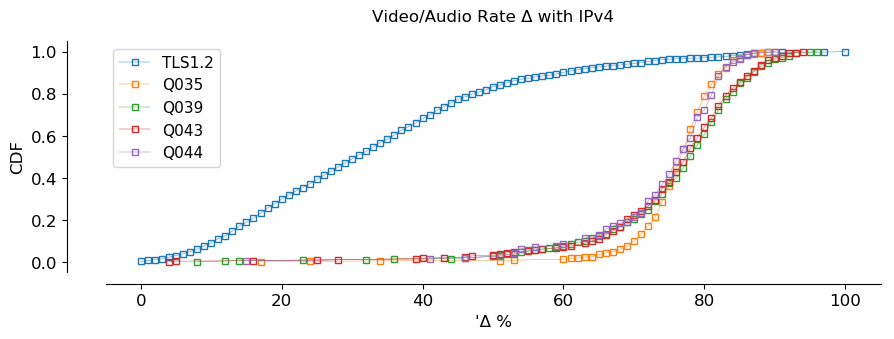
\includegraphics[width=\linewidth]{./plots/youtube/munich/graph_rate_diff.png}
    \end{subfigure}    
    \caption{CDF of video/audio rate difference in \% for IPv4 in Bhubaneswar, India and Munich, Germany}\label{fig:cdf-of-video-audio}
\end{figure}

%\end{frame}
%\clearpage
%
%\begin{frame}
%\shiftedframetitle{YouTube QoE}
%\begin{figure}[!htb]
%    
%    \begin{subfigure}{0.45\textwidth}
%        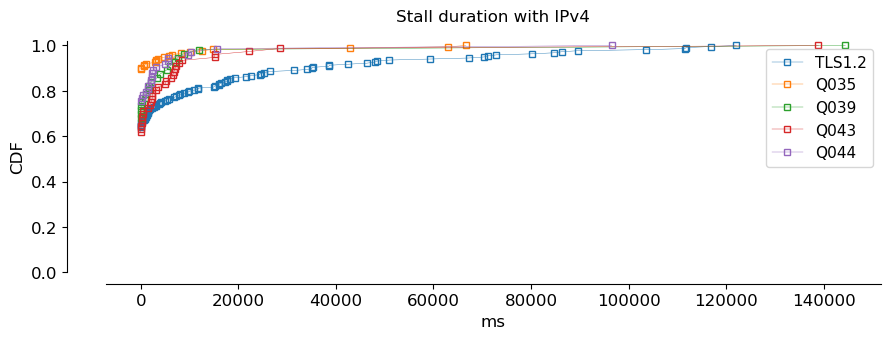
\includegraphics[width=\linewidth]{./plots/youtube/india/graph_stall_durations.png}
%    \end{subfigure}
%    \begin{subfigure}{0.45\textwidth}
%        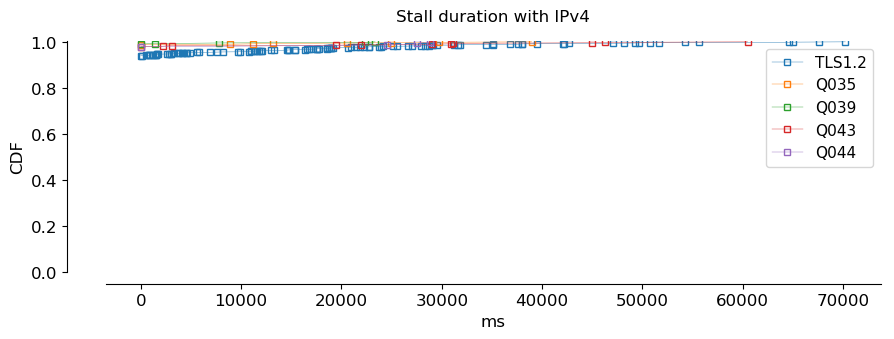
\includegraphics[width=\linewidth]{./plots/youtube/munich/graph_stall_durations.png}
%    \end{subfigure}    
%    \caption{CDF of stall durations for IPv4 in Bhubaneswar, India and Munich, Germany}\label{fig:cdf-of-stall}
%\end{figure}
\end{frame}
\clearpage
\begin{frame}
\shiftedframetitle{Throughput}

\begin{figure}[!htb]
    \begin{subfigure}{0.45\textwidth}
        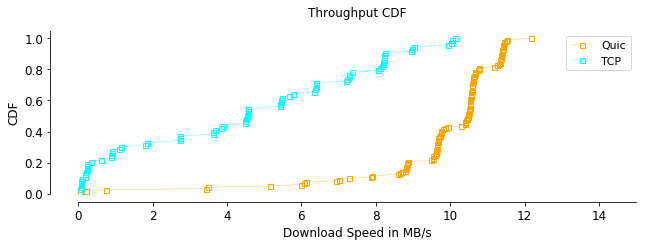
\includegraphics[width=\linewidth]{./plots/youtube/throughput/ThroughputCDF.png}
    \end{subfigure}   
%    \caption{CDF of Throughput of QUIC(Q044) and TCP downloading a YouTube video.}
%\end{figure}
%\begin{figure}[!htb]
    \begin{subfigure}{0.45\textwidth}
        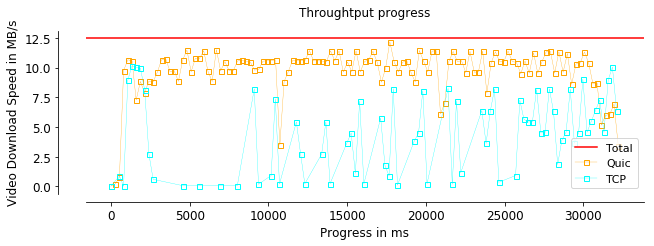
\includegraphics[width=\linewidth]{./plots/youtube/throughput/Throughtputprogress.png}
    \end{subfigure}  
    \caption{CDF of Throughput and Throughput of QUIC(Q044) and TCP downloading a YouTube video.}\label{fig:throughput-of-quic-q044-}
\end{figure}
%\end{frame}
%\clearpage
%
%\begin{frame}
%\shiftedframetitle{Throughput}
\begin{figure}[!htb]
    \begin{subfigure}{0.45\textwidth}
        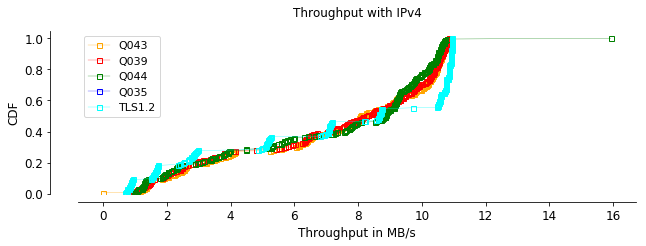
\includegraphics[width=\linewidth]{./plots/PI/gdrive/Throughput_ipv4.png}
    \end{subfigure}   
%    \caption{CDF of Throughput of QUIC(Q044, Q043, Q039) and TCP downloading files of different sizes from Google Drive}\label{fig:cdf-of-throughput}
%\end{figure}
%\begin{figure}[!htb]
%    \centering
    \begin{subfigure}{0.45\textwidth}
        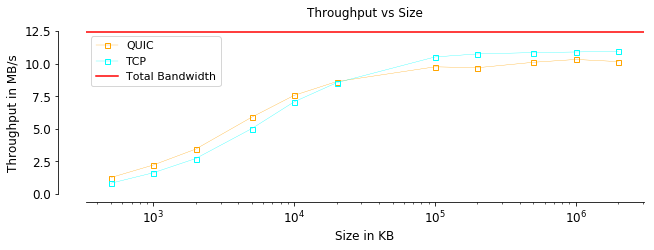
\includegraphics[width=\linewidth]{./plots/PI/gdrive/MeanThroughputvssize.png}
    \end{subfigure}   
    \caption{CDF of Throughput and Mean Throughput of QUIC(Q044, Q043, Q039) and TCP downloading files of different sizes from Google Drive}\label{fig:cdf-of-mean}
\end{figure}
\end{frame}
\clearpage

\begin{frame}
\shiftedframetitle{Fairness}
\begin{figure}[!htb]
    \begin{subfigure}{0.45\textwidth}
        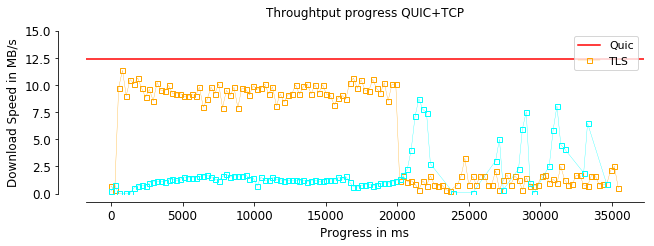
\includegraphics[width=\linewidth]{./plots/youtube/throughput/ThroughtputprogressQUIC+TCP.png}
    \end{subfigure}   
%    \caption{Throughput of 1 QUIC and 1 TCP concurrent flow with the download progress of a 30 second YouTube video}\label{fig:throughput-of-1}
%\end{figure}
%\begin{figure}[!htb]
    \begin{subfigure}{0.45\textwidth}
        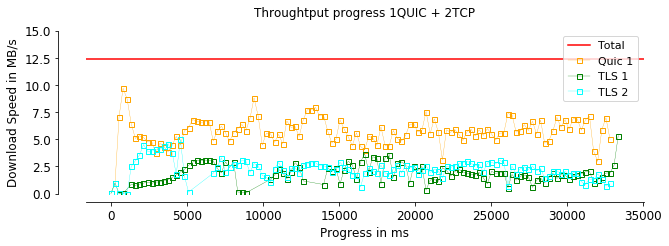
\includegraphics[width=\linewidth]{./plots/youtube/throughput/Throughtputprogress1QUIC+2TCP.png}
    \end{subfigure}
    \caption{Throughput of 1 QUIC and 1 TCP, 1 QUIC and 2 TCP concurrent flow with the download progress of a 30 second YouTube video}\label{fig:throughput-of-2}
\end{figure}

%\end{frame}
%\clearpage
%
%\begin{frame}
%\shiftedframetitle{Fairness}

\begin{figure}[!htb]
    \begin{subfigure}{0.45\textwidth}
        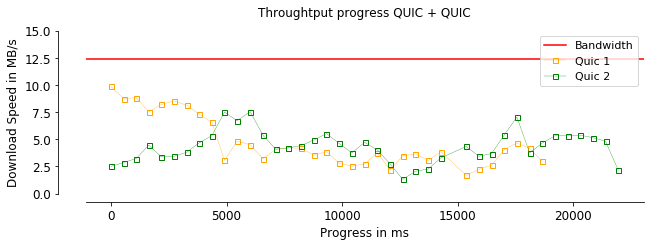
\includegraphics[width=\linewidth]{./plots/PI/throughput/ThroughtputprogressQUIC+QUIC.png}
    \end{subfigure}  
%    \caption{Throughput of 2 QUIC flows with the download progress of a 200 MB file from Google Drive}\label{fig:throughput-of-2y}
%\end{figure}
%\begin{figure}[!htb]
    \begin{subfigure}{0.45\textwidth}
        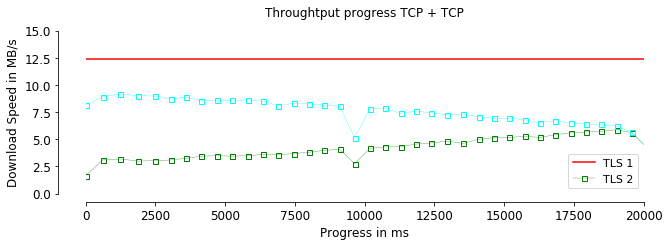
\includegraphics[width=\linewidth]{./plots/PI/throughput/ThroughtputprogressTCP+TCP.png}
    \end{subfigure}    
    \caption{Throughput of 2 QUIC flows and 2 TCP flows with the download progress of a 200 MB file from Google Drive}\label{fig:throughput-of-2g}
\end{figure}

\end{frame}
\clearpage

\begin{frame}
\shiftedframetitle{Fairness}
\begin{figure}[!htb]
    \begin{subfigure}{0.5\textwidth}
        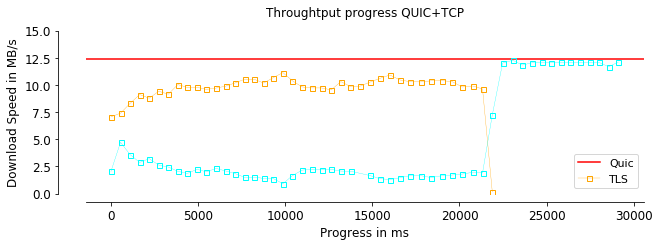
\includegraphics[width=\linewidth]{./plots/PI/throughput/ThroughtputprogressQUIC+TCP.png}
    \end{subfigure}
    %\caption{Throughput of 1 QUIC and 1 TCP flow with the download progress of a 200 MB file from Google Drive}\label{fig:throughput-of-2go}
%\end{figure}
%\begin{figure}[!htb]
    \begin{subfigure}{0.5\textwidth}
        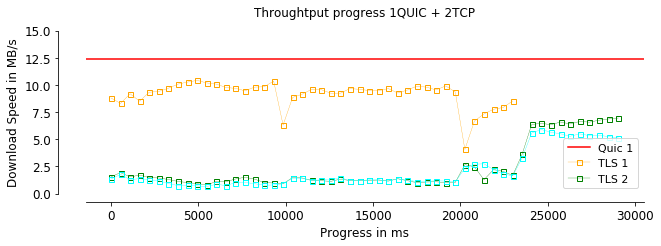
\includegraphics[width=\linewidth]{./plots/PI/throughput/Throughtputprogress1QUIC+2TCP.png}
    \end{subfigure}
    %\caption{Throughput of 1 QUIC and 2 TCP flow with the download progress of a 200 MB file from Google Drive}\label{fig:throughput-of-c}
%\end{figure}
%
%\end{frame}
%\clearpage
%
%\begin{frame}
%\shiftedframetitle{Fairness}
%\begin{figure}[!htb]
%    \centering
    \begin{subfigure}{0.5\textwidth}
        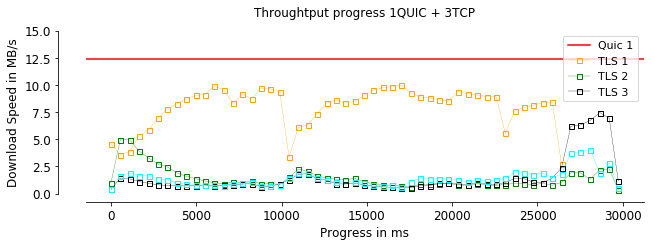
\includegraphics[width=\linewidth]{./plots/PI/throughput/Throughtputprogress1QUIC+3TCP.png}
    \end{subfigure}    
    \caption{Throughput of 1 QUIC and Multiple TCP flow with the download progress of a 200 MB file from Google Drive}
\end{figure}
\end{frame}
\clearpage

\begin{frame}
\shiftedframetitle{CPU Utilization}

\begin{figure}[!htb]
    \centering
    \begin{subfigure}{0.45\textwidth}
        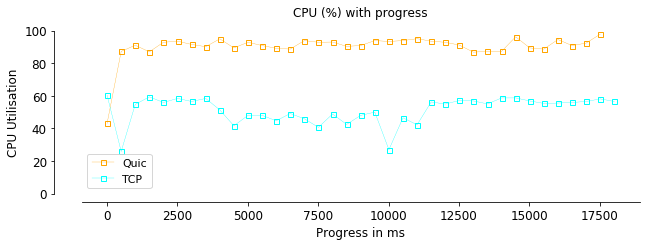
\includegraphics[width=\linewidth]{./plots/PI/cpu/cpupercentprogress.png}
    \end{subfigure}
    
    \caption{CPU utilization of QUIC(Q044) and TCP downloading a 200 MB file from Google Drive}\label{fig:cpu-utilization-of}
\end{figure}

%\end{frame}
%\clearpage
%
%\begin{frame}
%\shiftedframetitle{Scatter Plot Throughput vs CPU}

\begin{figure}[!htb]
    \centering
    \begin{subfigure}{0.45\textwidth}
        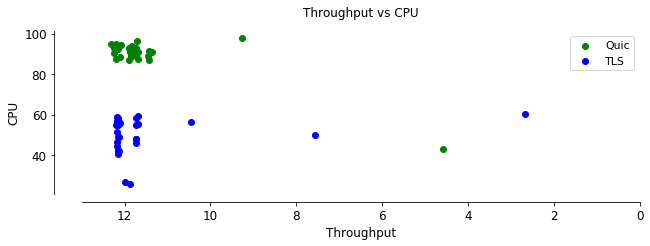
\includegraphics[width=\linewidth]{./plots/PI/throughputvscpu/ThroughputvsCPU.png}
    \end{subfigure}
    
    \caption{Scatter Plot for Throughput and CPU for QUIC and TCP while downloading from Google Drive}\label{fig:scatter-plot-for}
\end{figure}

\end{frame}
\clearpage

\begin{frame}
\shiftedframetitle{QUIC Profiling}
\begin{table}[ht]
    \begin{tabular}{@{}|l|l|l|l|l|l|@{}}
        \toprule
        \textbf{index} & \textbf{\%time} & \textbf{seconds} & \textbf{usecs/call} & \textbf{calls} & \textbf{syscall} \\ \midrule
        0              & 76.89           & 1.949677         & 24                  & 80800          & recvmsg          \\ \midrule
        1              & 17.33           & 0.439416         & 201                 & 2191           & epoll\_wait      \\ \midrule
        2              & 4.79            & 0.121456         & 57                  & 2141           & sendmsg          \\ \midrule
        3              & 0.22            & 0.005475         & 57                  & 96             & brk              \\ \midrule
        4              & 0.18            & 0.004439         & 2220                & 2              & poll             \\ \midrule
        5              & 0.08            & 0.00201          & 53                  & 38             & open             \\ \midrule
        6              & 0.08            & 0.001954         & 43                  & 45             & read             \\ \midrule
        7              & 0.07            & 0.001712         & 54                  & 32             & mmap2            \\ \midrule
        8              & 0.05            & 0.001261         & 53                  & 24             & mprotect         \\ \midrule
        9              & 0.05            & 0.001185         & 41                  & 29             & close            \\ \midrule
        10             & 0.03            & 0.000878         & 38                  & 23             & fstat64          \\ \bottomrule
    \end{tabular}
    \caption{Top-10 system calls for QUIC while downloading file from Google drive}\label{table:top-10-system-calls}
\end{table}
QUIC uses a maximum packet size of 1350 for IPv4 and 1370 for IPv6 to avoid packet fragmentation. Thus QUIC has to make many calls to send/recv system calls.
\end{frame}
\clearpage

\begin{frame}
\shiftedframetitle{QUIC Profiling}

\begin{figure}[!htb]
    \centering
    \begin{subfigure}{0.8\textwidth}
        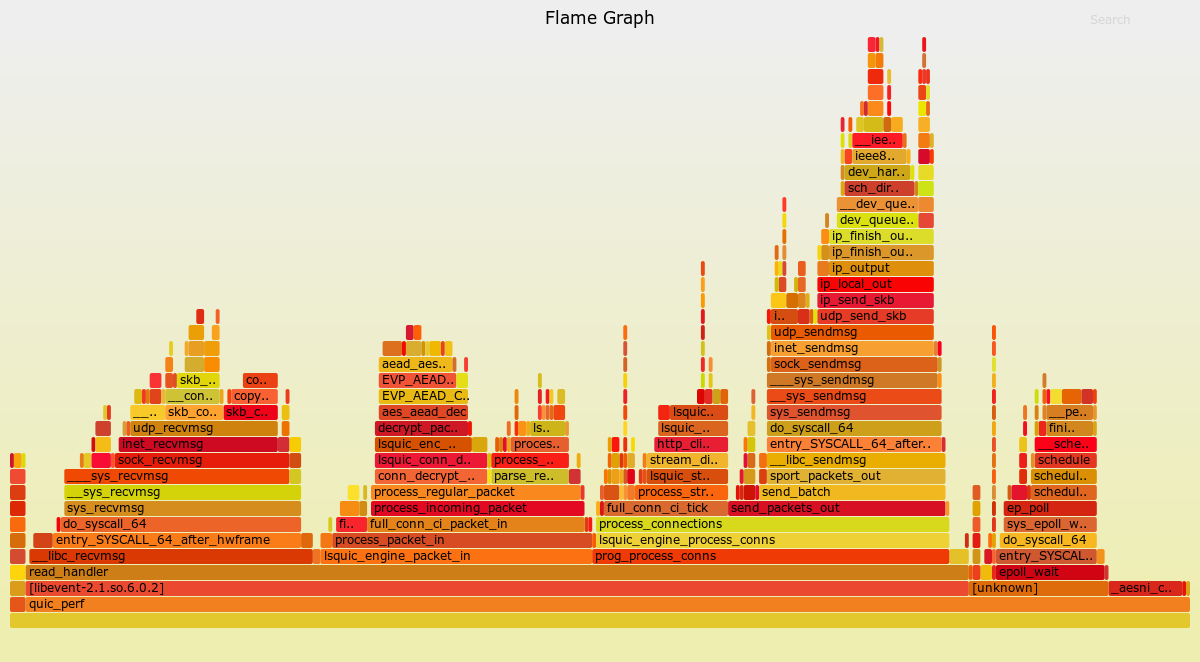
\includegraphics[width=\linewidth]{./plots/perf_flame_graphs/quic/kernel.png}
    \end{subfigure}
    
    \caption{CPU Flame Graph, showing codepaths that are consuming CPU cycles and by how much}\label{fig:cpu-flame-graph-}
\end{figure}
We can see that the width of the \_\_sys\_recvmsg and \_\_sys\_sendmsg is quite large indicating a lot of cpu usage in these paths. In case of UDP packets have to travel all the way up the stack.
\end{frame}
\clearpage

%\begin{frame}
%\shiftedframetitle{QUIC Discovery with Alt-Svc header and IETF QUIC}
%
%\begin{table}[ht]
%    \begin{tabular}{@{}|l|l|@{}}
%        \toprule
%        \textbf{QUIC Versions} & \textbf{No. of Websites returning Alt-Svc} \\ \midrule
%        35,39,43,44            & 1145                                       \\ \midrule
%        35,37,38,39            & 433                                        \\ \midrule
%        35,39,43               & 202                                        \\ \midrule
%        35,39                  & 3                                          \\ \midrule
%        39                     & 2                                          \\ \bottomrule
%    \end{tabular}
%    \caption{QUIC versions in Alt-Svc Header}\label{fig:quic-versions-in}
%\end{table}

%\end{frame}
%\clearpage
%
%\begin{frame}
%\shiftedframetitle{IETF QUIC}

%\begin{figure}[!htb]
%    \centering
%    \begin{subfigure}{0.45\textwidth}
%        \includegraphics[width=\linewidth]
%        {./plots/VM/ietf/handshake_times_ietf_ipv4.png}
%    \end{subfigure}
%    \caption{\label{fig:handshake_times_ietf_ipv4}Handshake IETF QUIC draft-17 ipv4}
%\end{figure}
%
%\begin{figure}[!htb]
%    \centering
%    \begin{subfigure}{0.45\textwidth}
%        \includegraphics[width=\linewidth]
%        {./plots/VM/ietf/handshake_times_ietf_ipv6.png}
%    \end{subfigure}
%    \caption{\label{fig:handshake_times_ietf_ipv6}Handshake IETF QUIC draft-17 ipv6}
%\end{figure}

%\begin{figure}[!t]
%    \centering
%    \begin{subfigure}{0.4\textwidth}
%        \includegraphics[width=\linewidth]
%        {./plots/VM/ietf/handshake_times_ietf_0rtt.png}
%    \end{subfigure}
%    \caption{\label{fig:handshake_times_0rtt_ipv4}Handshake IETF QUIC draft-17 0-rtt}
%\end{figure}
%
%\end{frame}
%\clearpage

\begin{frame}
\shiftedframetitle{Conclusion}
    \begin{itemize}
    \itemsep2em
    %\item When analyzing the connection establishment times for different versions of QUIC, in case of IPv4 we found that at 90th percentile Q044 performs slightly better by about 55 ms. As expected QUIC performs better than TLS 1.2 and TLS 1.3. At 50th percentile QUIC versions have similar latency but lower than TLS 1.2 by 34 ms and TLS 1.3 by 77 ms.
%In case of IPv6 all of the QUIC versions have quite similar values. Difference with TLS 1.2 remains similar to IPv4 but TLS 1.3 has lower connection times than TLS 1.2. But when we analyze Time to first byte we see that QUIC loses some of the improvements gained by 1-RTT connection times, it is still faster than TLS. At 50th percentile Q035, Q039, Q043 have a TTFB of around 206 ms, Q044 has a TTFB of 211 ms, TLS 1.2 has a TTFB of 261 ms and TLS 1.3 has a TTFB of 360 ms. Difference in total download time is similar to TTFB.

\item QUIC outperforms TLS in connection establishment times for both IPv4 and IPv6.

%\item QUIC loses some of its advantage when it comes to Time to first byte.

\item From the measurements done in India we find greater improvements for QUIC over TCP/TLS than in Munich which shows that benefits of QUIC is more evident in low-bandwidth, high-loss networks and high-RTT regions. 

%QUIC provides improvements of 240 ms, 340 ms over TLS 1.2, TLS 1.3 respectively at 75th percentile in India while it provides improvements of 210 ms, 245 ms over TLS 1.2, TLS 1.3 respectively in Munich for connection establishment time. These measurements are only for IPv4.

\item Q044 may have slightly better Connection times but TTFB and download time between different QUIC versions is similar for IPv4.

%\item For IPv6 QUIC versions perform similarly.

%\item In case of Video content delivery over YouTube, QUIC provides much better improvements in India than in Germany for Connect Time, Prebuffering time, Startup delay.

\item Overall download rate in case of Video content delivery for TLS 1.2 is higher than QUIC.
% and download rate for Q035 is higher than other QUIC versions for both India and Germany. But the difference between the download speeds is lesser in India than Germany. All observations are on IPv4 only. 

%In case of Video content delivery over YouTube, QUIC provides much better improvements in India than Germany for Connect Time, with an improvement of 550 ms at 50th percentile  over TLS, for Germany the value is 410 ms. For Prebuffering time, the gap between QUIC and TLS is 447 ms in Munich and 600 ms in India. 
%For Startup delay, the gap between QUIC and TLS is 665 ms in Munich and 861 ms in India.
%Overall download rate for TLS 1.2 is higher than QUIC and download rate for Q035 is higher than other QUIC versions for both India and Germany. But the difference between the download speeds is lesser in India than Germany. All observations are on IPv4 only. 

\item Q035 has higher download rates and lesser stall durations than other QUIC versions.

\item Google AS serves an overwhelming majority of the websites using QUIC, almost half of the websites in our target list. Only 5 ASes account for 85\% of our target websites.

%\item EDGECAST AS performs better than GOOGLE AS on connection establishment times, at 50th percentile it performs about 12 ms better. For TTFB gap between GOOGLE and EDGECAST increases to 144 ms. 

%\item EDGECAST doesn't support QUIC over IPv6 where GOOGLE has a clear advantage. 
%Connection times for GOOGLE - Google LLC, OVH - OVH SAS, IHCRU - Internet-Hosting Ltd are 36.556, 98.33, 201.959 respectively at the 50th percentile.

%GOOGLE AS having the largest amount of websites by quite a margin in our sample means that overall plots of our metrics mimic those of GOOGLE. But on closer inspection we can see that other ASes may perform better than GOOGLE. Looking at each individual AS more minutely we find that different QUIC versions perform similarly for GOOGLE, EDGECAST and OVH whereas for ICHPU and A2 HOSTING Q044 performs slightly better in terms of connection establishment times.

\end{itemize}
\end{frame}
\clearpage

\begin{frame}
\shiftedframetitle{Conclusion}
\begin{itemize}
    \itemsep2em
%\item In case of downloading a video from YouTube we find that both QUIC and TCP start  with the same throughput but QUIC maintains it over the entire duration of the download, TCP on the other hand has many peaks and falls. Mean throughput of QUIC is over twice that of TCP.%(9.70 MB/s to 4.43 MB/s)
\item Mean throughput of QUIC is over twice that of TCP.

\item QUIC performs better than TCP for smaller file sizes but for larger file sizes TCP has higher throughput.

\item CPU utilization in case of QUIC is almost twice that of TCP% while downloading large files from GDrvive.

\item QUIC sends most of its time in the kernel on expensive sendmsg/recvmsg system calls. 

\item QUIC grabs more than its fair share of bandwidth when it is competing with TCP. QUIC flows are fair to other QUIC flows and TCP flows are fair to other TCP flows.% Even with 2 and 3 competing TCP flows, QUIC maintains its mean bandwidth usage.

%\item Mean bandwidth usage of QUIC is more than twice the combined mean bandwidth usage of TCP. Though both TCP and QUIC use the same CUBIC congestion control algorithm, QUIC has been known to aggressively increase its congestion window size so it is able to grab most of the bandwidth more quickly. 

\end{itemize}
\end{frame}
\clearpage


\begin{frame}
\shiftedframetitle{Future work and limitations}
\begin{itemize}
\itemsep2em    
%    \item Geographical bias due to location of probes.For more representative results the tests should be deployed at multiple locations with the help of CAIDA Ark \cite{CAIDAArk} measurement infrastructure and SamKnows project\cite{SamKnowsproject}
%    
%    \item Mobile devices are a major source of QUIC traffic so tests need to be adopted for mobile devices using cronet\cite{cronet}.
%    
%    \item No support for 0-RTT connections in lsquic at the time of test creation. Support has been introduced in latest release.
%    
%    \item The QUIC \texttt{YouTube tests} have a higher failure rate than TCP \texttt{YouTube tests} which can be looked into.
%    
%    \item Other features of QUIC like Congestion control window size, Packet pacing, Flow control can be evaluated.
%    
%    \item  QUIC tests can be performed under constrained conditions like low buffer size, introducing random bandwidth changes, random packet loss and different RTTs.
%    
%    \item  Other metrics like no. of retransmissions, no. of packets lost, congestion window size can be measured.
%    
%    \item IETF QUIC may be standardized soon, it may also be considered for comparison with Google QUIC and TCP/TLS.
    \item For more representative results the tests should be deployed at multiple locations with the help of CAIDA Ark \cite{CAIDAArk} and SamKnows project\cite{SamKnowsproject}

\item Adopt tests need for mobile devices using cronet\cite{cronet}.

\item No support for 0-RTT connections in lsquic at the time of test creation. Support has been introduced in latest release.

\item The QUIC \texttt{YouTube tests} have a higher failure rate than TCP \texttt{YouTube tests} 

\item Other metrics like Congestion control window size and Packet pacing, no. of retransmissions, no. of packets lost. 

\item  Tests under constrained conditions like low buffer size, introducing random bandwidth changes, random packet loss and different RTTs.

%\item  Other metrics like no. of retransmissions, no. of packets lost, congestion window size can be measured.

%\item IETF QUIC may be standardized soon, it may also be considered for comparison with Google QUIC and TCP/TLS.
\item Adopt the tests for IETF QUIC

\end{itemize}
\end{frame}
\clearpage

\begin{frame}
\shiftedframetitle{Reproducibility}
\begin{itemize}
   \itemsep3em      
 \item The code is located in github repositories YouTube tests\cite{youtubetests}, quic\_perf\cite{quicp}, tls\_perf\cite{tlsp}.
 
 
 \item The data and jupyter notebooks used for analysis are present on the VM \textit{vmott16} and the github repository\cite{analysis}.
 
 \item Analysis for YouTube QoE has been done with scripts in \cite{thesis_repository}
    
\end{itemize}
\end{frame}
\clearpage

\begin{frame}
\shiftedframetitle{Prior Work}\label{prior_work}
    Langley et al. \cite{DBLP:conf/sigcomm/LangleyRWVKZYKS17} discuss about motivations in various design decisions of QUIC, development and testing performed over various iterations, performance improvements. They provide us with the first large-scale measurements of QUIC across various versions.
    
    Nepomuceno et al.\cite{8538687}, Cook et al.\cite{DBLP:conf/icc/CookMTH17} look at page load time.
    
    Li et al.\cite{DBLP:conf/pam/LiCJC18}, Kharat et al.\cite{8524247}, Qian et al. \cite{DBLP:journals/access/QianWT18}, Kakhki et al.\cite{DBLP:conf/imc/KakhkiJCNM17}look at throughput, congestion control and fairness among flows.
    
    Yu et al. \cite{DBLP:conf/ipccc/YuXY17} focused mainly on packet pacing mechanism for congestion control.
    
    Saverimoutou et al.\cite{DBLP:conf/iscc/SaverimoutouMV17}, Fischlin et al.\cite{DBLP:conf/ccs/FischlinG14} and Vaere et al.\cite{DBLP:conf/imc/VaereBKT18} look into the security aspects of QUIC.
    
    Willem et al.\cite{udpgso} and Edeline et al. \cite{DBLP:journals/corr/EdelineKTAD16} look into how QUIC being built on top of UDP affects it.
    
    Wang et al.\cite{DBLP:conf/mswim/WangBRP18} implement QUIC in the linux kernel and perform experiments to compare both in kernel mode.

    Rüth et al.\cite{DBLP:conf/pam/RuthPDH18} look into QUIC usage in the wild.

    
\end{frame}
\clearpage